\PassOptionsToPackage{colorlinks=true,linkcolor=blue,citecolor=blue,urlcolor=blue}{hyperref}
% REQ-FILE: The above line, \PassOptionsToPackage{} must be very first line.

\documentclass[11pt]{article}

% Encoding and font setup for cross-platform reproducibility
\usepackage[utf8]{inputenc}
\usepackage[T1]{fontenc}
\usepackage{lmodern}

% Improve readability for dense theoretical material
\usepackage{setspace}
\onehalfspacing

% Mathematical notation and table formatting for formal semantics
\usepackage{amsmath, amssymb}
\usepackage{booktabs}
\usepackage{bookmark}
\usepackage{graphicx}

% Theorem environments for definitions, lemmas, and formal statements
\usepackage{amsthm}

% plain style is italic body text (for theorems, lemmas, etc.)
\theoremstyle{plain}
\newtheorem{theorem}{Theorem}[section]
\newtheorem{lemma}[theorem]{Lemma}
\newtheorem{proposition}[theorem]{Proposition}
\newtheorem{corollary}[theorem]{Corollary}
\newtheorem{conjecture}[theorem]{Conjecture}

% definition style = upright body text (for definitions, examples)
\theoremstyle{definition}
\newtheorem{definition}[theorem]{Definition}
\newtheorem{example}[theorem]{Example}

% remark style = upright, lighter weight (for remarks, notes)
\theoremstyle{remark}
\newtheorem{remark}[theorem]{Remark}
\newtheorem{note}[theorem]{Note}

% Bibliography management and hyperlink support
\usepackage{url}
\usepackage{hyperref}
\usepackage{natbib}

% Support multiple author affiliations
\usepackage{authblk}

% Improve typographic quality and line breaking
\usepackage{microtype}

% Categorical and commutative diagrams
\usepackage{tikz}
\usepackage{tikz-cd}
\usetikzlibrary{arrows.meta,calc,fit,positioning,shapes.geometric}

% Callout boxes for examples and emphasis
\usepackage{mdframed}
\usepackage[most]{tcolorbox}

% Keywords macro for structured abstract metadata
\providecommand{\keywords}[1]{\textbf{Keywords: } #1}

% Notation for Raw vs Canonical categories in CEP/CEE
\newcommand{\Raw}{\mathsf{Raw}}
\newcommand{\Canon}{\mathsf{Canon}}

% Reusable figure callout box for visual emphasis
\newcommand{\FigureCallout}[2]{%
  \begin{tcolorbox}[
    colback=gray!5,
    colframe=black!40,
    title={#1},
    fonttitle=\bfseries,
    arc=3pt,
    boxrule=0.5pt,
    width=\linewidth,
    enhanced,
    breakable
  ]
  #2
  \end{tcolorbox}
}

% Paragraph spacing prioritizes readability over traditional indentation
\setlength{\parskip}{0.75em}
\setlength{\parindent}{0em}

% Compact list formatting for dense conceptual content
\usepackage{enumitem}
\setlist[itemize]{itemsep=0.2em, topsep=0.2em, parsep=0em, partopsep=0em}

% Defensive re-definition ensures commands exist if loaded earlier
\providecommand{\Raw}{\mathrm{Raw}}
\providecommand{\Canon}{\mathrm{Canon}}

\title{A Bicategorical Semantics of Civic Explanations and Vertical Domains}

\author[1,2]{Denise Case}
\affil[1]{Northwest Missouri State University, Computer Science and Information Systems, Maryville, MO, USA}
\affil[2]{Civic Interconnect, Ely, MN, USA}

\date{\today}

\begin{document}

\maketitle
\vspace{-1em}

% Explicitly mark preprint status
\begin{tcolorbox}[colback=gray!10, colframe=black!20, boxrule=0.3pt]
  \textbf{Preprint Notice.}
  This preprint has not undergone peer review.
  It is shared to support community discussion, transparency research,
  and early technical evaluation.
\end{tcolorbox}

\begin{abstract}
  The Civic Exchange Protocol (CEP) provides a canonical substrate for
  civic entities, relationships, and exchanges.
  The Contextual Evidence and Explanations (CEE) layer extends this
  substrate with structured, evidence-based explanations of why
  particular civic decisions, alerts, or highlights occur.
  This paper develops a geometric and categorical perspective on the
  combined CEP+CEE architecture.
  We introduce the notion of a \emph{vertical domain} as a structured
  slice through the global civic graph, and show how verticals compose
  into a stack with a bicategorical semantics:
  objects as entities, 1-morphisms as relationships plus provenance,
  and 2-morphisms as explanations that relate one morphism-level
  interpretation to another.
  The resulting framework is mathematically tidy yet operationally
  useful: it supports interoperable modeling across domains such as
  SME-friendly procurement, community asset access, environmental
  compliance, education access, and disaster resilience, while making
  the logic of explanations explicit and reusable.
\end{abstract}

\begin{keywords}
  Civic data;
  category theory;
  functorial data modeling;
  interoperability;
  canonicalization;
  identifiers;
  provenance.
\end{keywords}

% !TeX root = 00P1_cae_ontology.tex

\section{Introduction and Motivation}
\label{sec:introduction}

Civic systems are governed by complex interactions among laws, institutions,
infrastructure, financial flows, and measured outcomes.
Data describing these systems is typically fragmented across domains such as procurement, public
health, environmental regulation, education, and infrastructure.
While each domain is often supported by mature data systems, the structural relationships
that connect authority, obligation, action, and long-term outcomes are
rarely represented in a unified or
interoperable form~\cite{bowker2000sorting,edwards2011infrastructure}.

This fragmentation presents a fundamental obstacle to accountability and
longitudinal analysis.
Short-term metrics are frequently privileged over
long-term public value, and outcomes that accrue over decades—such as population
health, infrastructure resilience, or environmental quality—are difficult to
relate back to the legal, institutional, and financial decisions that shape
them~\cite{edwards2011infrastructure,kahn2002information}.
As a result, public investments with high upfront costs and diffuse
benefits are systematically undervalued, even when their historical impact is
well established.

Many existing approaches focus either on transactional data (such as payments
or contracts), legal texts (such as statutes and regulations), or outcome
measures (such as health or economic indicators).
Few provide a principled way to connect these elements without
collapsing distinct concepts into a single
layer or embedding interpretive assumptions directly into data models~\cite{bowker2000sorting}.

This paper introduces the Civic Accountable Entities (CAE) ontology as a
foundational response to this challenge.
CAE defines a formal ontology of entities that participate in
obligations, authority, and accountability within civic systems.
Rather than modeling domains or sectors directly, CAE identifies
a small set of disjoint entity kinds that are stable across time and context and
sufficient to represent the structural relationships underlying civic accountability.

The design of CAE emphasizes ontological clarity over descriptive completeness.
Entities are partitioned into disjoint kinds with explicit identity criteria;
roles, classifications, and sectoral labels are modeled as attributes or
relationships rather than as entity kinds.
This discipline prevents ontological overlap and supports formal reasoning
about obligations, authority, and evidence.

CAE draws on foundational work in formal ontology, particularly the
emphasis on rigorous categorization found in BFO~\cite{smith2015bfo} and
DOLCE~\cite{masolo2004wonderweb}, while making commitments tailored to
civic accountability: entities are included in CAE only insofar as they
participate in accountability-bearing relationships, and the ontology
is designed to remain stable as domains, policies, and tooling evolve.
Section~\ref{sec:related} discusses these relationships in detail.

CAE provides the ontological foundation for the Civic Exchange Protocol (CEP),
which models how entities exchange value and authority, and for Contextual
Evidence and Explanations (CEE), which attaches structured explanations to
civic decisions.
By separating what exists from how it moves and how decisions are explained,
CAE enables interoperable, auditable, and longitudinal analysis of public
systems while remaining neutral with respect to policy positions or causal claims.

The remainder of this paper is organized as follows:
Section~\ref{sec:related} situates CAE within related work in formal ontology;
Section~\ref{sec:principles} outlines the design principles and scope
of CAE;
Section~\ref{sec:ontology} defines the six disjoint entity kinds;
Section~\ref{sec:relationships} discusses relationships and structural constraints;
Section~\ref{sec:evaluation} evaluates CAE via competency questions;
Section~\ref{sec:laws} discusses laws, regulations, and accountability chains;
Section~\ref{sec:outcomes} discusses outcomes, observations, and public value;
Section~\ref{sec:discussion} includes discussion and future work;
and Section~\ref{sec:conclusion} provides a conclusion.
       % Introduction
% !TeX root = 00P3_cee_verticals.tex
\section{Background}
\label{sec:background}

This section summarizes the ingredients on which our framework rests:
the Civic Exchange Protocol (CEP), the Contextual Evidence and
Explanations (CEE) layer, and the categorical tools we draw upon.

\subsection{The Civic Exchange Protocol (CEP)}

CEP is a schema- and rewriting-based specification for civic data.
At a high level, CEP defines:
\begin{itemize}[nosep]
  \item \emph{Entity schemas} for units such as municipalities, facilities,
        tenders, lots, contracts, programs, shelters, and so on;
  \item \emph{Relationship schemas} for links such as buyer--issues--tender,
        asset--located-in--area, facility--has--permit;
  \item \emph{Exchange and record-envelope schemas} that bundle entities
        and relationships with provenance and validation artifacts;
  \item \emph{Vocabularies} for shared codes (procedure types, violation
        types, status codes, etc.);
  \item \emph{Canonicalization and identity rules} that normalize data and
        compute stable fingerprints such as SNFEI.
\end{itemize}

The operational specification and reference implementation are maintained
in the open-source \emph{Civic Interconnect} project~\citep{cep2025spec},
which also defines concrete schemas, vocabularies, and adapters for
multiple domains (campaign finance, municipalities, environment,
education, and procurement).
We refer the reader to the companion CEP theory paper for the underlying
theory of rewriting, canonical forms, graph normalization, and identity
fingerprints, which builds on standard accounts of term rewriting
systems~\citep{baader1998term,terese2003rewriting}.

\subsection{Contextual Evidence and Explanations (CEE)}

CEE is a nascent but structurally constrained layer that sits above CEP.
Conceptually, CEE introduces three core artifacts:
\begin{description}
  \item[Evidence sets] summarizing the facts, metrics, and features that
        support a particular decision or classification.
  \item[Attribution sets] describing which models, rules, pipelines, and
        agents are responsible for that decision.
  \item[Explanation bundles] packaging evidence, attribution, and
        narrative fields for a specific subject entity or graph.
\end{description}

An explanation bundle is always anchored to one or more CEP entities or
relationships, and to an explicit \emph{explanation type}, such as:
\begin{itemize}[nosep]
  \item SME-friendly procurement lot;
  \item Priority neighborhood for community asset investment;
  \item Elevated environmental compliance risk facility;
  \item High-value education program for a given learner profile;
  \item Critical shelter or route in a resilience plan.
\end{itemize}
In this way, CEE does not operate over arbitrary raw data, but over
canonicalized CEP graphs.
This dependency is central to the semantic structure developed later:
explanations are layered \emph{on top of} canonical entities and
relationships, and they inherit their invariants from the underlying
canonicalization and identity rules.

\subsection{Category Theory and Categorical Semantics}

At a technical level, we appeal to standard notions from category theory
and bicategory theory.
Good general references include Mac~Lane's classic treatment of
categories~\citep{maclane1998categories},
modern introductions by Awodey~\citep{awodey2010category},
Leinster~\citep{leinster2014basic},
and Riehl~\citep{riehl2017category},
and applied accounts such as
Spivak's work on functorial data modeling and migration
\citep{spivak2013functorial,spivak2014category}
and Fong and Spivak's ``Seven Sketches''~\citep{fong2019seven}.
We assume familiarity with:
\begin{itemize}[nosep]
  \item categories, functors, and natural transformations;
  \item monoidal structure and composition of morphisms;
  \item bicategories, 2-morphisms, and coherence conditions.
\end{itemize}
Appendix~\ref{app:A} provides a brief, self-contained
review of the categorical notions we rely on, and Appendix~\ref{app:E}
offers a glossary-oriented view for non-specialists.

Informally, we will use the following guiding intuition:
\begin{itemize}
  \item CEP canonical graphs form (at least) a category: objects are
        canonical entities or graphs; morphisms are relationships and
        validated transformations between them.
  \item CEE explanations behave like 2-morphisms: they ``sit between''
        morphisms, refining or annotating one morphism with respect to
        another.
\end{itemize}
This is enough to motivate a bicategorical semantics without committing
to a fully formalized construction in this paper.
The remainder of the paper builds on this background to develop the
notion of vertical domains and their bicategorical structure.
  % Background and preliminaries
% !TeX root = 00P3_cee_verticals.tex

\section{Recap of the CEP Canonical Layer}
\label{sec:cep-recap}

The first paper in this series develops CEP as a rewriting-based,
categorical framework for civic data.
Here we briefly recap the aspects that are most relevant for
vertical domains and civic explanations.

% ------------------------------------------------------------
\subsection{Canonical Entities and Relationships}
% ------------------------------------------------------------

Let $\mathcal{E}$ denote the collection of CEP entity schemas, and
$\mathcal{R}$ the collection of relationship schemas.
Each entity instance is normalized by a strategy-controlled rewriting
system that:
\begin{itemize}[nosep]
  \item canonicalizes lexical forms (names, addresses, codes);
  \item aligns fields with schema-defined structures;
  \item resolves identifiers and computes SNFEI-style fingerprints.
\end{itemize}

The result is a set of canonical entities and relationships that can be
treated as objects and morphisms in a category we denote by
$\mathbf{CEP}$.

% ------------------------------------------------------------
\subsection{Graphs, Envelopes, and Provenance}
% ------------------------------------------------------------

CEP records live not in isolation but as graphs: entities linked by
relationships, wrapped in record envelopes that carry provenance and
validation evidence.
The canonical encoding specification (CEC) and graph normalization
specification (GNS) ensure that equivalent graphs normalize to identical
representations and hashes.

For the purposes of this paper, it is enough to view:
\begin{itemize}
  \item \emph{Objects} of $\mathbf{CEP}$ as canonical entity-graph
        components (possibly with envelopes attached);
  \item \emph{Morphisms} as (typed) relationships, exchanges, or
        validated graph transformations between such components.
\end{itemize}

% ------------------------------------------------------------
\subsection{Adapters as Functorial Bridges}
% ------------------------------------------------------------

Adapters map raw data from external sources into the canonical CEP
universe.
Each adapter:
\begin{enumerate}[nosep]
  \item canonicalizes the input (lexical and semantic normalization);
  \item aligns it to CEP schemas;
  \item computes identities and attaches attestations.
\end{enumerate}

Operationally, an adapter behaves like a functor from a ``source
category'' of raw records to the target category $\mathbf{CEP}$.
In the first paper, this is treated primarily at the level of rewriting
and graph semantics; here we build on that intuition to organize
vertical domains.
         % Recap of CEP canonical layer
% !TeX root = 00P3_cee_verticals.tex

\section{Vertical Domains}
\label{sec:verticals}

Informally, practitioners already speak of ``verticals'': procurement
verticals, health verticals, education verticals, and so on.
In most software settings these labels refer to application silos or
product lines.
In the CEP+CEE setting we adopt a more structural definition.

\begin{definition}[Vertical domain]
  A \emph{vertical domain} \(V\) consists of three interlocking
  components:
  \begin{enumerate}[label=(\alph*)]
    \item A \emph{CEP scope} \(C_V\): a selected subset of CEP schemas,
          vocabularies, and identifier schemes, together with the
          induced rewriting and identity rules on the corresponding
          entity and relationship objects.
    \item An \emph{adapter scope} \(A_V\): a set of deterministic
          adapters that map one or more raw data sources into canonical
          CEP entities and relationships within \(C_V\).
    \item A \emph{CEE scope} \(E_V\): a family of explanation types,
          evidence-set schemas, and attribution-set schemas that attach
          structured explanations to entities and relationships in
          \(C_V\).
  \end{enumerate}
\end{definition}

Intuitively, \(C_V\) specifies \emph{what in the civic universe we
  are looking at}; \(A_V\) specifies \emph{how raw data enters that
  universe}; and \(E_V\) specifies \emph{why certain parts of that
  universe are highlighted as important}.
A vertical is therefore not merely an application domain but a
\emph{sustained lens} on the canonical civic graph.

\paragraph{Examples.}

\begin{itemize}
  \item A \textbf{SME-friendly procurement} vertical might include
        entities for buyers, tenders, lots, contracts, and suppliers;
        relationships describing which buyer issues which tender and
        which contract is awarded to which supplier; adapters from
        OCDS-style procurement releases into that schema; and CEE
        explanation types that answer questions such as ``Why is this
        lot SME-friendly?''.
  \item A \textbf{community asset access} vertical might include
        entities for public assets (parks, libraries, recreation
        centres), neighbourhoods, and jurisdictions; relationships
        placing assets into neighbourhoods and neighbourhoods into
        jurisdictions; adapters from city open data portals and
        population grids; and explanations that answer ``Why is this
        neighbourhood prioritized for new assets?''.
\end{itemize}

In both cases the vertical is defined by a \emph{coherent pattern of
  use} across CEP, adapters, and CEE, not by any single file or schema.

\paragraph{Design constraints.}

Vertical domains are subject to several design constraints that
distinguish them from one-off analyses:

\begin{enumerate}[label=(\roman*)]
  \item \textbf{Reusability.}  The CEP scope \(C_V\) should reuse
        existing canonical schemas and vocabularies wherever possible,
        rather than proliferating bespoke types.
  \item \textbf{Determinism.}  Adapters in \(A_V\) must respect CEP's
        canonicalization and identity rules so that repeated runs
        produce stable entity identifiers and graph structure.
  \item \textbf{Legibility.}  Explanations in \(E_V\) must satisfy
        CEE's evidence and attribution constraints, so that their
        semantics are inspectable, testable, and comparable across
        instances and time.
  \item \textbf{Locality.}  Each vertical should be cancellable or
        extensible with minimal disruption to others: one can remove
        the community asset vertical without affecting the SME
        procurement vertical, and vice versa.
\end{enumerate}

These constraints are reflected in the repository structure: each
vertical has its own \emph{about} file, examples, adapters, and tests,
but they all sit on top of the same CEP and CEE foundations.
They ensure that verticals compose cleanly into a larger civic data
ecosystem.
   % Vertical domains
% !TeX root = 00P3_cee_verticals.tex

\section{The Stack of Vertical Domains}
\label{sec:stack}

Although vertical domains can be developed independently, they share a
common architectural pattern.
We describe this pattern as a \emph{stack} layered over the CEP base.

% ------------------------------------------------------------
\subsection{Layers of the Stack}
% ------------------------------------------------------------

Conceptually, the stack has four layers:
\begin{enumerate}[label=(\arabic*),nosep]
  \item \textbf{Canonical base (CEP).}
        Schemas, vocabularies, identity,
        canonicalization, and graph normalization.
  \item \textbf{Adapters.}
        Deterministic mappings from raw sources into
        CEP entities and relationships.
  \item \textbf{Explanations (CEE).}
        Explanation types, evidence sets,
        attribution sets, and narratives over canonical graphs.
  \item \textbf{Vertical domains.}
        Slices that select subsets of the
        above three layers for specific civic questions.
\end{enumerate}

The first three layers are domain-agnostic:
they apply to any civic context expressible in CEP.
The fourth layer instantiates them for
particular questions of interest.

% ------------------------------------------------------------
\subsection{Verticals as Fibers over the CEP Universe}
% ------------------------------------------------------------

Let $\mathcal{U}_{\mathrm{CEP}}$ denote the ``universe'' of CEP schemas
and vocabularies.
Each vertical $V$ chooses a subset
$\mathcal{U}_V \subseteq \mathcal{U}_{\mathrm{CEP}}$
together with adapters and explanations.

The collection of all verticals can be
arranged as a family of fibers over
$\mathcal{U}_{\mathrm{CEP}}$:
\[
  \pi : \mathsf{Vert} \to \mathcal{U}_{\mathrm{CEP}},
\]
where the fiber over a given subset of schemas is the set of verticals
that use exactly those schemas (up to specified equivalence).

We do not formalize this as a fibration in the categorical sense,
but the analogy is useful:
moving along the base corresponds to changing
which parts of CEP are in scope;
moving within a fiber corresponds to changing
explanations or adapters while keeping the same schemas.

% ------------------------------------------------------------
\subsection{Reusability Across Verticals}
% ------------------------------------------------------------

A major benefit of the stack perspective is reusability.
Because verticals share the CEP base,
several components can be reused:

\begin{itemize}
  \item entity schemas (e.g., municipalities, regions, facilities)
        may appear in multiple verticals;
  \item identity schemes (e.g., SNFEI)
        provide cross-vertical linking;
  \item vocabularies (e.g., procedure types, violation types)
        can be shared;
  \item explanation types may be reused or adapted
        across verticals.
\end{itemize}

This manifests as maps between vertical domains,
a topic we return to in Section~\ref{sec:bicat}
and Section~\ref{sec:cases}.
       % Stack of vertical domains
% !TeX root = 00P3_cee_verticals.tex

\section{A Bicategorical Semantics of Civic Explanations}
\label{sec:bicat}

We now sketch a bicategorical semantics that integrates CEP and CEE.
The goal is not a fully formal construction, but a coherent picture that
makes vertical domains and their interconnections mathematically
transparent.

% ------------------------------------------------------------
\subsection{CEP as a Category of Canonical Civic Graphs}
% ------------------------------------------------------------

Let $\mathbf{CEP}$ be the category whose:
\begin{itemize}[nosep]
  \item objects are canonical CEP graphs
        (entities, relationships, envelopes, identity, and provenance)
        modulo graph normalization;
  \item morphisms are well-typed graph homomorphisms and
        schema-respecting transformations,
        composed by ordinary function composition.
\end{itemize}

Adapters are then functors
$F : \mathcal{C} \to \mathbf{CEP}$
from source categories $\mathcal{C}$ of raw records.

For a vertical $V$, we restrict to a subcategory
$\mathbf{CEP}_V \subseteq \mathbf{CEP}$
as in Section~\ref{sec:verticals}.

% ------------------------------------------------------------
\subsection{CEE Explanations as 2-Morphisms}
% ------------------------------------------------------------

Explanations in CEE relate not only objects but \emph{morphisms}.
Informally:
\begin{itemize}
  \item A relationship, classification, or decision is represented by a
        morphism $f : X \to Y$ in $\mathbf{CEP}_V$.
  \item An explanation bundle describes why $f$ holds,
        which evidence it depends on,
        and which agents or models are responsible.
\end{itemize}

Given two morphisms $f,g : X \to Y$
(for example, two different ways of classifying the same lot or facility),
an explanation can be understood as a 2-morphism
\[
  \alpha : f \Rightarrow g
\]
witnessing how $f$ is obtained from $g$
under a particular explanatory contract,
or how $f$ is justified relative to a baseline.

This motivates the following heuristic construction.

\begin{conjecture}
  There exists a bicategory $\mathbf{Civ}$ whose:
  \begin{itemize}
    \item objects are canonical civic graphs
          (or families of entities);
    \item 1-morphisms are CEP relationships and graph transformations
          with provenance;
    \item 2-morphisms are CEE explanations relating 1-morphisms
          under explanation types and contracts.
  \end{itemize}
\end{conjecture}

We do not claim to have constructed $\mathbf{Civ}$ in full generality,
but the vertical domains we study can be understood as fragments of such
a bicategory.

% ------------------------------------------------------------
\subsection{Verticals as Sub-bicategories}
% ------------------------------------------------------------

For each vertical $V$, we may consider the full sub-bicategory
$\mathbf{Civ}_V$ of $\mathbf{Civ}$ whose:
\begin{itemize}[nosep]
  \item objects are those graphs built from $\mathcal{E}_V$
        and $\mathcal{R}_V$;
  \item 1-morphisms are CEP morphisms in $\mathbf{CEP}_V$;
  \item 2-morphisms are explanations in $\Xi_V$
        attaching to those morphisms.
\end{itemize}

This aligns with the architectural view of Section~\ref{sec:stack}:
each vertical is a slice of the full bicategory,
with its own adapters and explanation types.

% ------------------------------------------------------------
\subsection{Maps Between Vertical Domains}
% ------------------------------------------------------------

Once we acknowledge this bicategorical structure,
maps between verticals become semantically meaningful.
For verticals $V$ and $W$ we can study:

\begin{itemize}
  \item \emph{Entity alignment functors}
        $F : \mathbf{CEP}_V \to \mathbf{CEP}_W$
        that identify shared entity types
        (e.g., municipalities, regions, facilities).
  \item \emph{Evidence transport}
        that lifts metrics or indices from one vertical to another
        (e.g., deprivation indices used in both health
        and community asset explanations).
  \item \emph{Explanation composition}
        where 2-morphisms in $\mathbf{Civ}_V$
        and $\mathbf{Civ}_W$ compose to yield a joint explanation
        (e.g., combining SME-friendly procurement
        with local economic impact).
\end{itemize}

These constructions are sketched in more concrete form in
Section~\ref{sec:cases}.
       % Bicategorical semantics
% !TeX root = 00P3_cee_verticals.tex
\section{Maps Between Vertical Domains}
\label{sec:maps}

Once vertical domains are regarded as structured slices of a common
bicategorical space, it becomes natural to ask how they relate to one another.
In this section we sketch three classes of ``maps between verticals'',
each corresponding to a different way of transporting structure.

\subsection{Entity-Alignment Functors}

The most basic maps are functors that align entities across verticals.
%
For instance, the same municipality may appear in both the community
asset vertical and the environmental compliance vertical.
%
Both verticals use the same CEP entity schema and the same SNFEI
identifier, but they emphasise different relationships and
explanations.

An \emph{entity-alignment functor} between verticals \(V\) and \(W\)
is a functor \(F : \mathcal{C}_V \to \mathcal{C}_W\) between the
underlying entity-relationship categories such that:

\begin{itemize}
  \item on objects, \(F\) identifies shared entities (e.g.\ a
        municipality in \(V\) with the same municipality in \(W\));
  \item on morphisms, \(F\) preserves those relationships that are
        meaningful in both verticals (e.g.\ jurisdictional embeddings).
\end{itemize}

These functors formalize the intuition that verticals live in the
same universe; they differ in focus, not in ontological commitment.

\subsection{Evidence-Transport Maps}

A richer kind of map transports \emph{evidence semantics} from one
vertical to another.
%
For example, a deprivation index used in the community asset vertical
may also be relevant in a health outcomes vertical, or risk metrics
computed in an environmental compliance vertical may inform a
resilience vertical.

Given verticals \(V\) and \(W\), an \emph{evidence-transport map}
associates to each explanation type in \(V\) a compatible explanation
type or evidence schema in \(W\), together with transformation rules
for metric names, scales, and interpretations.
%
At the bicategorical level, such a map can be viewed as a 2-functor
that acts on explanation 2-morphisms.

\subsection{Explanation-Composition Maps}

Finally, explanations from different verticals can sometimes be
composed to yield higher-level narratives.
%
For instance:

\begin{itemize}
  \item An SME-friendly procurement explanation may be composed with a
        community asset explanation to yield an account of why a
        particular procurement decision supports community economic
        resilience.
  \item An environmental risk explanation may be composed with a
        shelter-criticality explanation to express how facility risk
        impacts evacuation planning.
\end{itemize}

We refer to such constructions as \emph{explanation-composition
  maps}.
%
Formally, they appear as higher-order 2-morphisms that combine
explanations from different verticals along shared objects and
relationships.

These maps are central to the idea of a civic \emph{stack}: they show
how verticals remain modular while still participating in a coherent
global semantics.
        % Maps between vertical domains
% !TeX root = 00P3_cee_verticals.tex
\section{Illustrative Case Studies of Vertical Domains}
\label{sec:cases}

We briefly illustrate how the preceding ideas manifest in concrete
verticals.
Each case study is treated schematically; detailed schemas
and examples are available in the accompanying implementation.

\subsection{SME-Friendly Procurement}

The SME procurement vertical $V_{\mathrm{SME}}$ selects:
\begin{itemize}[nosep]
  \item entities: buyers, tenders, lots, contracts, suppliers;
  \item relationships: buyer--issues--tender, tender--has--lot,
        contract--awarded-to--supplier, and so on;
  \item adapters: mappings from OCDS-style releases to CEP entities;
  \item explanation types: SME-friendly procurement explanations
        attached to lot entities.
\end{itemize}
The primary question is:
\begin{quote}
  Why is this lot considered SME-friendly?
\end{quote}
Evidence includes lot value relative to a threshold, procedure type, lot
structure, and possibly historical SME participation.
Attribution identifies the rule or model version and responsible agents.

In bicategorical terms, SME-friendly explanations are 2-morphisms in
$\mathbf{Civ}_{\mathrm{SME}}$ that refine classifications of lots.
They enable functorial comparison across jurisdictions and time.

\subsection{Community Asset Access}

The community asset vertical $V_{\mathrm{Assets}}$ selects:
\begin{itemize}[nosep]
  \item entities: assets (parks, libraries), areas, jurisdictions;
  \item relationships: asset--located-in--area, area--part-of--jurisdiction;
  \item adapters: from open data portals and population grids;
  \item explanation types: area access priority explanations.
\end{itemize}
The primary question is:
\begin{quote}
  Why is this neighborhood prioritized for investment in community assets?
\end{quote}
Evidence aggregates population, distance to nearest assets, asset counts
within thresholds, and equity indices.
These explanations act as 2-morphisms over morphisms 
that connect areas to assets and jurisdictions.

\subsection{Environmental Compliance, Education Access, and Resilience}

Similarly structured verticals arise for environmental compliance,
education access and value, and disaster resilience.
In each case:
\begin{itemize}
  \item a subset of CEP schemas defines the entities and relationships;
  \item adapters bring public data into canonical form;
  \item explanations attach to highlighted entities or relationships,
        answering a focused ``why'' question.
\end{itemize}
Across these verticals, common entities (e.g., municipalities) and
indices (e.g., deprivation measures) appear repeatedly, enabling maps
between sub-bicategories and composition of explanations.

These case studies illustrate how vertical domains instantiate the
abstract framework of bicategories of explanations, providing
structured, interpretable insights tailored to specific civic questions.

       % Illustrative case studies
% !TeX root = 00P3_cee_verticals.tex


\section{Related Work}
\label{sec:related}

We briefly situate this work within three strands of literature:
interoperability specifications, explainable AI, and categorical
semantics.

\subsection{Interoperability Specifications}

CEP is inspired in part by standards such as OCDS for procurement,
FHIR for health data, and PROV for provenance.
These specifications establish domain-specific schemas and sometimes limited notions of
provenance and interpretation.
CEP extends this tradition with a rewriting-based canonicalization layer and unified identity semantics.

The notion of vertical domains resonates with how profiles and
extensions are used in these communities but adds an explicit semantic
stack and categorical framing.

\subsection{Explainable AI and Model Governance}

CEE is aligned with work on model cards, data statements, and regulatory
requirements for explanation in domains such as credit, employment, and
public benefits.
However, most existing approaches treat explanations
as annotations of model artifacts, not as 2-morphisms over canonical civic graphs.
Our approach suggests a more structural integration of explanations with data semantics.

\subsection{Categorical Semantics and Applied Category Theory}

Finally, this work connects to applied category theory in databases,
open games, probabilistic programming, and causal inference.
The idea of treating explanations as 2-morphisms is reminiscent of compositional
approaches to lenses, rewrites, and double categories.
We view this paper as an invitation to bring similar tools to civic data and
governance contexts.
     % Related work
% !TeX root = 00P3_cee_verticals.tex

\section{Research Agenda}
\label{sec:agenda}

The preceding sections outline a conceptual framework.
Turning this into a mature theory and a robust body of practice
requires sustained work along several fronts.
Here we sketch a research agenda structured around three themes:
formalization, empirical validation, and tooling.

% ------------------------------------------------------------
\subsection{Formalization}
% ------------------------------------------------------------

On the formal side, several questions arise naturally:

\begin{itemize}
  \item \textbf{Bicategory structure.}
        Precisely characterize the bicategory of civic entities,
        relationships, and explanations.
        %
        Specify identity and composition laws for 2-morphisms and
        prove coherence theorems.
  \item \textbf{Vertical domains as fibres.}
        Develop a fibration or indexed-category perspective in which
        each vertical domain appears as a fibre over a base of CEP
        schemas and vocabularies.
  \item \textbf{Transport of explanations.}
        Characterize when explanations in one vertical can be
        transported to another via functors and 2-functors between
        corresponding categories.
  \item \textbf{Universal properties.}
        Investigate whether certain verticals satisfy universal
        properties (limits, colimits, adjunctions) with respect to
        others, especially in multi-criteria decision settings.
\end{itemize}

These questions are not merely abstract.
They capture when and how explanations can be safely reused, compared,
or composed across domains.

% ------------------------------------------------------------
\subsection{Empirical Validation}
% ------------------------------------------------------------

The framework must also be tested against real civic data and
realistic decision contexts.

\begin{itemize}
  \item \textbf{Case studies.}
        Develop detailed case studies for a small set of verticals
        (such as SME procurement and community asset access), tracing
        the entire pipeline from raw data through CEP, adapters, and
        CEE into concrete decisions.
  \item \textbf{Identity robustness.}
        Evaluate the stability and robustness of SNFEI identifiers and
        other identity schemes under noisy and adversarial naming
        conditions, since identity is central to cross-vertical
        reasoning.
  \item \textbf{Explanation quality.}
        Assess whether CEE-style explanations improve human
        understanding, trust, and decision quality compared to
        baseline dashboards or opaque scores.
  \item \textbf{Cross-vertical scenarios.}
        Design scenarios where decisions depend on combining
        information from multiple verticals, and study how well the
        proposed mapping and composition mechanisms behave.
\end{itemize}

% ------------------------------------------------------------
\subsection{Tooling and Automation}
% ------------------------------------------------------------

Finally, there is a practical tooling agenda.

\begin{itemize}
  \item \textbf{Vertical scaffolding.}
        Automate the creation of vertical scaffolds from compact
        \texttt{about.yaml} specifications, including directory
        layouts, adapter stubs, CEE helper modules, and example tests.
  \item \textbf{Schema- and vocab-aware IDE support.}
        Develop editor and CI tooling that keeps schemas, adapters,
        explanations, and vertical metadata in sync.
  \item \textbf{Visualization.}
        Create visualization tools that expose the geometric and
        categorical structure: civic graphs, explanation layers, and
        maps between verticals.
  \item \textbf{Reference implementations.}
        Maintain a small but representative library of open verticals
        that act as regression suites for both the theory and the
        tooling.
\end{itemize}

Together, these threads describe how the initial geometric and
bicategorical picture can grow into a stable, shared foundation for
civic data and civic explanations.
      % Research agenda
% !TeX root = 00P2_cep_semantics.tex


\section{Limitations and Future Work}
\label{sec:limitations}

The categorical core presented in this paper captures identity,
canonicalization, provenance, and interoperability for discrete,
revision-based civic records.
Several important extensions remain outside the present scope.

Many civic systems also generate data that is statistical, uncertain, or
continuously updated (e.g., longitudinal indicators, evolving aggregates).
Incorporating such information may require probabilistic semantics or
temporal indexing, which are not modeled in the current framework.

Jurisdictions evolve data models over time.
Although CEP supports adapters for structural variation,
a full account of schema evolution, including additions,
deprecations, and long-term migration paths, remains future work.

\paragraph{Multi-Stage and Nested Exchanges.}

Some workflows involve layered or multi-party processes
(e.g., multi-level budget allocations, nested reporting pipelines).
These may benefit from higher-structured categorical tools,
but such extensions lie beyond the scope of this foundational treatment.

\paragraph{Rule Sensitivity in Canonicalization.}

Certain linguistic cases (such as expansions of abbreviations like “S.A.”)
require stratified rule ordering within the normalization pipeline rather
than treating all rewrite rules as freely permutable.
This refinement does not affect the well-definedness of the canonicalization
function but does highlight the need for continued empirical tuning of rule strata.

\medskip

The present semantics establish a robust core for identity and interoperability.
Extending CEP to the richer data practices found across governments and civic ecosystems
is a key direction for future work.

% ------------------------------------------------------------
\section{Conclusion}
\label{sec:conclusion}

We presented a categorical semantics for the Civic Exchange Protocol
that unifies canonicalization, provenance, adapters, and context tags
into a coherent mathematical framework.
This perspective makes explicit the invariants that govern identity,
record evolution, and interoperability across heterogeneous civic data systems.

Canonicalization was formulated as a deterministic monoidal functor,
ensuring stable identifiers and well-defined equivalence classes.
Jurisdictional adapters were modeled as oplax functors, capturing how
local structure may be weakened while preserving global identity.
Context tags were expressed via a fibered category, isolating
interpretive annotations from canonical record content.
Together, these structures yield formal guarantees for identifier preservation,
compositional provenance, and cross-jurisdiction reconciliation.

The resulting semantics provides a rigorous foundation for validation,
verification, and future extensions of CEP.
It enables principled design of domain schemas, vocabularies,
and interoperability standards, while remaining extensible to evolving civic workflows.
As civic data ecosystems continue to grow in scale and complexity,
categorical methods offer a durable and expressive language for ensuring that shared
identities and exchanges remain consistent, transparent, and reliable.


\section*{Acknowledgements}

Portions of this work were developed through human-computer collaboration
using modern computational tools.
Generative language models were used to assist with editing, formatting,
and consistency checking during manuscript preparation.
All conceptual framing, formal development, results, interpretations, and conclusions
are the author's own.
All generated suggestions were critically reviewed and validated, and
the author takes full responsibility for the content of this work.  % Limitations, future work, conclusion

\appendix
\clearpage

% ============================================================
\appendix
\section*{Appendix A. Category-Theoretic Background}
\addcontentsline{toc}{section}{Appendix A. Category-Theoretic Background}
% ============================================================

This appendix summarizes the categorical notions used in the paper.
It is intended for readers with a background in data modeling,
databases, or formal methods who may not use category theory daily.
The goal is conceptual clarity rather than mathematical depth.

% ------------------------------------------------------------
\subsection*{A.1 Categories}
% ------------------------------------------------------------

A \emph{category} consists of:
\begin{itemize}
    \item a collection of \textbf{objects};
    \item a collection of \textbf{morphisms} (arrows) between objects;
    \item an associative composition operation
          and an identity arrow for each object.
\end{itemize}

Intuition:
\begin{itemize}
    \item Objects represent states or structured data (e.g., CEP records).
    \item Morphisms represent valid transformations (e.g., amendments).
    \item Composition corresponds to applying transformations sequentially.
\end{itemize}

\medskip
Example:
A sequence of record updates in CEP corresponds to a chain of morphisms
\[ R_0 \to R_1 \to R_2 \to \cdots. \]

% ------------------------------------------------------------
\subsection*{A.2 Functors}
% ------------------------------------------------------------

A \emph{functor} $F : \mathbf{C} \to \mathbf{D}$ maps:
\begin{itemize}
    \item each object of $\mathbf{C}$ to an object of $\mathbf{D}$,
    \item each morphism in $\mathbf{C}$ to a morphism in $\mathbf{D}$,
\end{itemize}
such that identities and composition are preserved.

Intuition:
\begin{itemize}
    \item A functor is a structure-preserving translation.
    \item CEP uses functors to model processes such as
          envelope construction or canonicalization.
\end{itemize}

% ------------------------------------------------------------
\subsection*{A.3 Natural Transformations}
% ------------------------------------------------------------

Given functors $F, G : \mathbf{C} \to \mathbf{D}$,
a \emph{natural transformation} $\eta : F \Rightarrow G$ assigns
to each object $X$ in $\mathbf{C}$ a morphism
\[
\eta_X : F(X) \to G(X)
\]
such that each square
\[
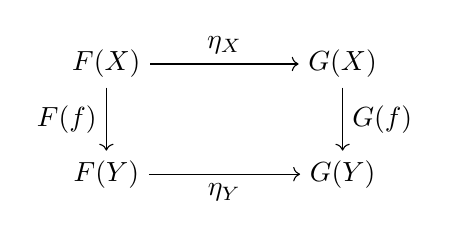
\begin{tikzpicture}[baseline=(current bounding box.center)]
\node (FX) at (0,0) {$F(X)$};
\node (GX) at (3,0) {$G(X)$};
\node (FY) at (0,-1.4) {$F(Y)$};
\node (GY) at (3,-1.4) {$G(Y)$};
\draw[->] (FX) -- node[above] {$\eta_X$} (GX);
\draw[->] (FY) -- node[below] {$\eta_Y$} (GY);
\draw[->] (FX) -- node[left] {$F(f)$} (FY);
\draw[->] (GX) -- node[right] {$G(f)$} (GY);
\end{tikzpicture}
\]
commutes for all morphisms $f : X \to Y$.

Intuition:
\begin{itemize}
    \item Naturality means: \emph{"attest first then transform" =
          "transform first then attest"}. 
    \item This is exactly the coherence needed for CEP attestation chains.
\end{itemize}

% ------------------------------------------------------------
\subsection*{A.4 Monoidal Categories}
% ------------------------------------------------------------

A \emph{monoidal category} is a category equipped with:
\begin{itemize}
    \item a tensor product $\otimes$ combining objects,
    \item a unit object $I$,
    \item coherence laws ensuring associativity and proper unit behavior.
\end{itemize}

In CEP, the relevant monoidal structure is \textbf{string concatenation}:
\begin{itemize}
    \item canonical components (name, address, date) combine via $\otimes$,
    \item the canonicalization functor preserves this structure strictly.
\end{itemize}

This allows the SNFEI to be treated as a universal construction.

% ------------------------------------------------------------
\subsection*{A.5 Oplax Functors}
% ------------------------------------------------------------

Given monoidal categories $(\mathbf{C}, \otimes)$ and $(\mathbf{D}, \otimes)$,
an \emph{oplax monoidal functor} $F : \mathbf{C} \to \mathbf{D}$ comes with
coherence maps
\[
F(X) \otimes F(Y) \to F(X \otimes Y)
\]
that need not be invertible.

Intuition:
\begin{itemize}
    \item Oplax functors allow \textbf{structure weakening}.
    \item This directly models jurisdictional adapters:
          some structure from the local schema may be incomplete or
          only partially mappable to the global vocabulary.
\end{itemize}

% ------------------------------------------------------------
\subsection*{A.6 Indexed Families and Fibrations}
% ------------------------------------------------------------

A \emph{fibration} $\pi : \mathbf{E} \to \mathbf{B}$ consists of:
\begin{itemize}
    \item a base category $\mathbf{B}$,
    \item a total category $\mathbf{E}$,
    \item a projection functor $\pi$,
    \item satisfying certain lifting properties.
\end{itemize}

The fiber over $B \in \mathbf{B}$ is the category
\[
\mathbf{E}_B = \{ E \in \mathbf{E} \mid \pi(E) = B \}.
\]

Intuition for CEP:
\begin{itemize}
    \item $\mathbf{B} = \mathbf{CEP}$ (identity-bearing records),
    \item $\mathbf{E} = \mathbf{CT}$ (records plus context tags),
    \item the fiber over $R$ is the set of all allowed context tags for $R$,
    \item fibers reindex naturally when $R$ evolves.
\end{itemize}

This formalizes the idea that context tags do not affect identity.

% ------------------------------------------------------------
\subsection*{A.7 Universal Properties (Informal)}
% ------------------------------------------------------------

A universal property specifies an object uniquely up to isomorphism
by the role it plays in relation to others.

In CEP:
\begin{itemize}
    \item the canonical string is universal for its admissible class
          of normalized components,
    \item the SNFEI is obtained by applying a hashing endofunctor,
    \item identity preservation follows from the uniqueness of the
          universal construction.
\end{itemize}

\bigskip
This concludes the appendix. Readers seeking more detail may consult
Mac~Lane~\cite{maclane1971categories},
Awodey~\cite{awodey2010category},
and Spivak~\cite{spivak2014category}.
   % Category background
% !TeX root = 00P3_cee_verticals.tex
\section*{Appendix B. Worked Examples}
\label{app:B}
\addcontentsline{toc}{section}{Appendix B. Worked Examples}

This appendix presents two concrete worked examples of bicategorical
interpretation: one for SME-friendly procurement and one for community
asset access.

\subsection*{B.1 SME-Friendly Procurement}

Consider a procurement lot with noisy inputs:
multiple spellings of the supplier's name,
ambiguous CPV codes,
and missing procedure-type metadata.

\paragraph{Step 1: Canonicalization (CEP base).}
\begin{enumerate}
  \item Normalize the entity fields (legal name, jurisdiction, value).
  \item Produce a canonical string in fixed order.
  \item Compute SNFEI via SHA-256.
\end{enumerate}

\paragraph{Step 2: Adapter semantics.}
Jurisdictional quirks (missing CPV codes, inconsistent currencies)
are handled via oplax functorial rules.

\paragraph{Step 3: CEE explanation.}
Evidence: low estimated value, open procedure type, minimal documentation.
Attribution: rule-based model ``sme-rule-v1''.
Narrative: ``This lot appears SME-friendly because \dots''.

Here the explanation is a 2-morphism refining the procurement relationship.

\subsection*{B.2 Community Asset Access}

Consider a neighborhood polygon and a dataset of parks and libraries.

Step 1: Construct CEP entities:
\begin{itemize}
  \item area entity (neighborhood),
  \item asset entities (parks, libraries),
  \item relationships linking assets to areas.
\end{itemize}

Step 2: Compute evidence layers and metrics:
population-served,
distance-to-assets,
equity index.

Step 3: Perform CEE prioritization:
Based on computed metrics and attribution model,
the vertical outputs a bundle with AREA\_ACCESS\_PRIORITY.
This bundle is a 2-morphism living above the area's incoming and
outgoing relationships.

\subsection*{B.3 Composition Across Verticals}

A municipality appearing in both verticals
supports functorial maps aligning their CEP entities and enabling
interoperable explanations.

   % Worked examples
% !TeX root = 00P1_cae_ontology.tex

\clearpage
\section*{Appendix C. Glossary of Terms}
\addcontentsline{toc}{section}{Appendix C. Glossary of Terms}



This appendix provides concise definitions of key terms used throughout the paper.

\subsection*{Entity Kinds}

\textbf{Actor (A):}
An entity capable of bearing rights, obligations, or responsibilities within
civic systems when acting as an accountable party.
Examples include governments, public agencies, businesses, nonprofits, and universities.

\textbf{Site/Asset (S):}
A physical or operational entity that is acted upon but does not bear obligations.
Examples include facilities, buildings, infrastructure, and power plants.

\textbf{Instrument (I):}
An enduring construct that creates, modifies, or constrains rights, obligations,
or authority.
Examples include statutes, regulations, contracts, grants, permits, and licenses.

\textbf{Event (E):}
A time-indexed occurrence asserted under the authority of an Instrument.
Examples include payments, inspections, filings, violations, and audits.

\textbf{Jurisdiction (J):}
An entity that scopes authority, applicability, and governance, defining where
Instruments apply and where Events occur.
Examples include nations, states, municipalities, and regulatory regions.

\textbf{Observation (O):}
A measurement or indicator describing state, performance, or outcomes.
Observations do not create obligations or authorize actions.
Examples include health outcomes, coverage rates, emissions intensity measures,
and educational attainment indicators.

\subsection*{Design Concepts}

\textbf{Accountability Analysis:}
The examination of relationships, obligations, and authority structures within
civic systems in order to make responsibility and oversight inspectable.

\textbf{Accountability-bearing Relationship:}
A relationship that establishes or reflects accountability obligations between
entities, such as delegation of authority, participation in an Event, or the
measurement of outcomes.

\textbf{Applied Ontology:}
The use of ontological methods and principles to structure, clarify, and analyze
real-world domains for practical purposes.

\textbf{Competency Questions:}
Questions that an ontology should be able to answer, used to guide its development
and to evaluate its adequacy for the intended domain.

\textbf{Completeness:}
The extent to which an ontology captures the concepts and relationships required
for its stated purpose, without implying exhaustive coverage of all possible phenomena.

\textbf{Disjointness:}
The property that entity kinds do not overlap;
each entity belongs to exactly one kind.

\textbf{Domain Ontology:}
An ontology that captures concepts and relationships specific to a particular
application domain.
CAE is not a domain ontology.

\textbf{Domain-Constrained Reference Ontology:}
An ontology that provides a stable, reusable set of entity kinds and relationships
tailored to a particular domain, without committing to sector-specific taxonomies.
CAE is a domain-constrained reference ontology.

\textbf{Enduring Entity:}
An entity that persists through time while maintaining its identity, even as its
properties or relationships change.

\textbf{Entity Kind:}
A fundamental category of entities within the ontology, defined by distinct
identity criteria and invariant over time.

\textbf{Longitudinal Change:}
Variation or trends in data, conditions, or outcomes observed over extended periods
of time.

\textbf{Knowledge Representation:}
The formal specification of entities, relationships, and structures within a domain
to support interoperability and structured analysis.

\textbf{Ontology:}
A formal representation of entities within a domain
and the relationships that hold between them.

\textbf{Ontology Drift:}
The gradual divergence of an ontology's scope, structure, or commitments
from its original design intent.

\textbf{Selective Modeling:}
The inclusion of entities based on operational relevance rather than exhaustive
enumeration, introducing entities only when they participate in
accountability-bearing relationships.

\textbf{Semantics:}
The interpretation of structures and relationships defined by an ontology, without
implying evaluative or causal claims at the ontological level.

\textbf{Soundness:}
The property that an ontology's definitions and constraints are internally
consistent and aligned with their intended interpretations.

\textbf{Subclassing:}
The creation of a hierarchy of classes or categories within an ontology,
where more specific classes inherit properties and relationships from more
general ones.
CEA avoids subclassing within its six entity kinds.

\textbf{Time-Indexed Entity:}
An entity whose identity or assertions are associated with specific points or
intervals in time.

\textbf{Upper Ontology:}
A domain-independent ontology intended to provide general categories applicable
across many domains.
CAE is not an upper ontology.

\subsection*{Instrument Roles (Descriptive)}

\textbf{Normative role (descriptive):}
A functional role in which an Instrument establishes authority or defines
obligations.
Examples include statutes, acts, and treaties.

\textbf{Regulatory role (descriptive):}
A functional role in which an Instrument specifies procedures, thresholds, or
requirements.
Examples include regulations, rules, and administrative codes.


\subsection*{Methodological Context}

CAE is a formal ontology in the knowledge representation tradition:
a specification of what kinds of entities exist in the civic accountability domain,
what properties they have, and what relationships hold between them.
The six entity kinds form a strict partition: each entity belongs to exactly one
kind, and kinds do not overlap.
This structure supports rigorous, neutral reasoning about obligations, authority,
and evidence without embedding causal or evaluative assumptions.
   % Proof sketches
% !TeX root = 00_cep_semantics.tex
\clearpage
\section*{Appendix D. Diagrammatic Intuition}
\addcontentsline{toc}{section}{Appendix D. Diagrammatic Intuition}

This appendix provides informal diagrams for the categorical structures
introduced in the main text.
The goal is to support intuition rather than to introduce new formal content.

% ------------------------------------------------------------
\subsection*{D.1 Morphisms in \texorpdfstring{$\mathbf{CEP}$}{CEP}}
% ------------------------------------------------------------

Figure~\ref{fig:cep-morphisms} depicts CEP objects as attested record
states and morphisms as provenance-preserving transformations.

\begin{figure}[ht]
  \centering
  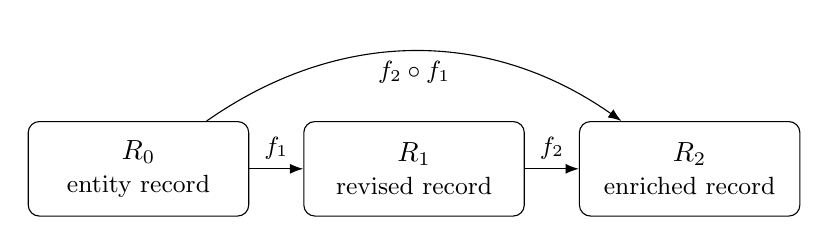
\begin{tikzpicture}[
      node distance=3.5cm,
      state/.style={rectangle,rounded corners,draw,minimum width=2.8cm,minimum height=1.2cm,align=center},
      >=Latex
    ]
    \node[state] (R0) {$R_0$\\{\small entity record}};
    \node[state,right of=R0] (R1) {$R_1$\\{\small revised record}};
    \node[state,right of=R1] (R2) {$R_2$\\{\small enriched record}};

    \draw[->] (R0) -- node[above]{\small $f_1$} (R1);
    \draw[->] (R1) -- node[above]{\small $f_2$} (R2);
    \draw[->, bend left=35]
    (R0) to node[below]{\small $f_2 \circ f_1$} (R2);
  \end{tikzpicture}

  \caption{Morphisms in $\mathbf{CEP}$ as provenance-preserving transformations.
    Each arrow corresponds to a valid record evolution that preserves schema
    validity, revision monotonicity, and canonical identity.}
  \label{fig:cep-morphisms}
\end{figure}

% ------------------------------------------------------------
\subsection*{D.2 Naturality of Attestations}
% ------------------------------------------------------------

Figure~\ref{fig:naturality-attestations} visualizes attestations as a
natural transformation between two envelope functors
$\mathcal{E}, \mathcal{E}' : \mathbf{P} \to \mathbf{E}$.

\begin{figure}[ht]
  \centering
  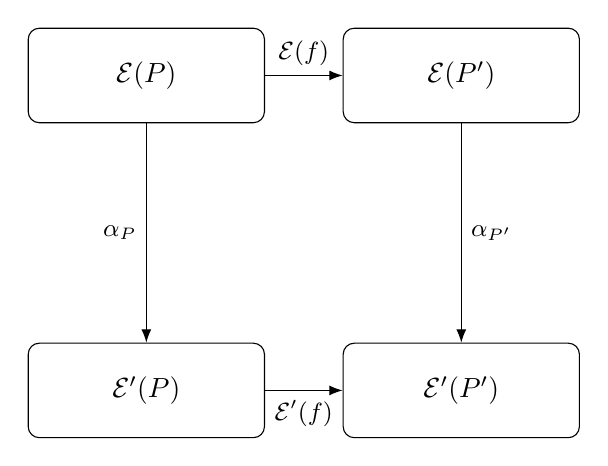
\begin{tikzpicture}[
      node distance=4.0cm,
      obj/.style={rectangle,rounded corners,draw,minimum width=3.0cm,minimum height=1.2cm,align=center},
      >=Latex
    ]
    \node[obj] (EP) {$\mathcal{E}(P)$};
    \node[obj,right of=EP] (EPP) {$\mathcal{E}(P')$};
    \node[obj,below of=EP] (E2P) {$\mathcal{E}'(P)$};
    \node[obj,below of=EPP] (E2PP) {$\mathcal{E}'(P')$};

    \draw[->] (EP) -- node[above]{\small $\mathcal{E}(f)$} (EPP);
    \draw[->] (E2P) -- node[below]{\small $\mathcal{E}'(f)$} (E2PP);
    \draw[->] (EP) -- node[left]{\small $\alpha_P$} (E2P);
    \draw[->] (EPP) -- node[right]{\small $\alpha_{P'}$} (E2PP);
  \end{tikzpicture}
  \caption{Naturality square for attestations.
    The equality
    $\alpha_{P'} \circ \mathcal{E}(f) = \mathcal{E}'(f) \circ \alpha_P$
    expresses that attestation commutes with valid transformations of payloads.}
  \label{fig:naturality-attestations}
\end{figure}

% ------------------------------------------------------------
\subsection*{D.3 Canonicalization Pipeline}
% ------------------------------------------------------------

Figure~\ref{fig:canonicalization-pipeline-appendix} summarizes the canonicalization
pipeline: normalization, assembly, and hashing.

\begin{figure}[ht]
  \centering
  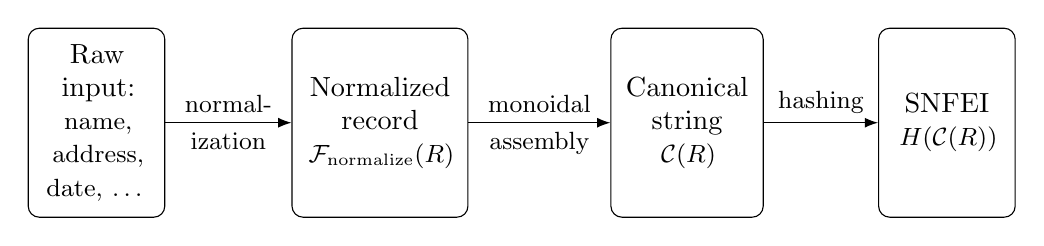
\begin{tikzpicture}[
      stage/.style={
          rectangle,
          rounded corners,
          draw,
          minimum width=1.5cm,
          minimum height=2.4cm,
          align=center
        },
      >=Latex
    ]
    % Explicit positions
    \node[stage, text width=1.5cm] at (0,0)   (raw)   {Raw input:\\{\small name, address, date, \dots}};
    \node[stage, text width=2cm] at (3.6,0) (norm)  {Normalized record\\{\small $\mathcal{F}_{\text{normalize}}(R)$}};
    \node[stage, text width=1.7cm] at (7.5,0)   (canon) {Canonical string\\{\small $\mathcal{C}(R)$}};
    \node[stage, text width=1.5cm] at (10.8,0) (hash) {SNFEI\\{\small $H(\mathcal{C}(R))$}};

    % Arrows from right edge to left edge
    \draw[->] (raw.east)   --
    node[above]{\small normal-}
    node[below]{\small ization}
    (norm.west);
    \draw[->] (norm.east) --
    node[above]{\small monoidal}
    node[below]{\small assembly}
    (canon.west);
    \draw[->] (canon.east) -- node[above]{\small hashing}  (hash.west);
  \end{tikzpicture}
  \caption{The canonicalization pipeline as a composition of a
    normalization functor, a strict monoidal assembly functor, and a
    hashing endofunctor that collapses canonical strings to identifiers.}
  \label{fig:canonicalization-pipeline-appendix}
\end{figure}


% ------------------------------------------------------------
\subsection*{D.4 Jurisdictional Adapters as Oplax Functors}
% ------------------------------------------------------------

Figure~\ref{fig:oplax-adapter-appendix} illustrates the weakened coherence
condition for an oplax functor
$\mathcal{A} : \mathbf{J_{local}} \to \mathbf{J_{global}}$.

\begin{figure}[ht]
  \centering
  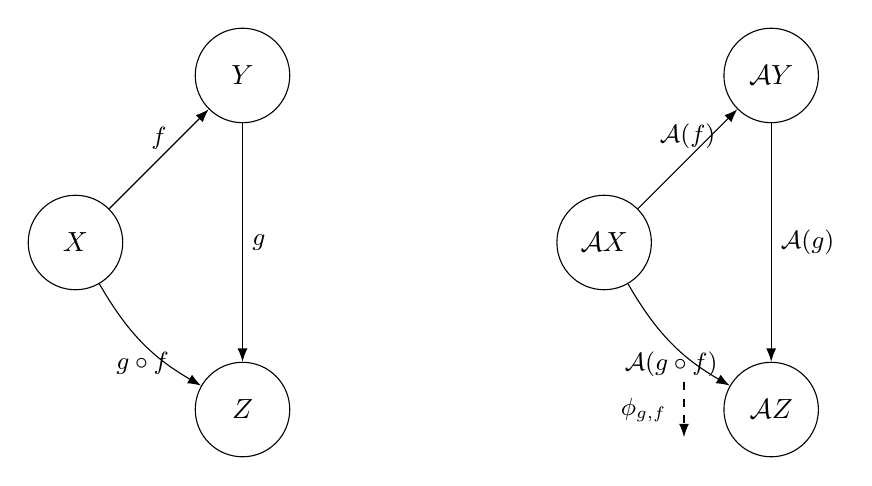
\begin{tikzpicture}[
      node distance=3.0cm,
      obj/.style={circle,draw,minimum size=1.2cm,align=center},
      >=Latex
    ]
    % Local side
    \node[obj] (X) {$X$};
    \node[obj,above right of=X] (Y) {$Y$};
    \node[obj,below right of=X] (Z) {$Z$};

    \draw[->] (X) -- node[above]{\small $f$} (Y);
    \draw[->] (Y) -- node[right]{\small $g$} (Z);
    \draw[->,bend right=15] (X) to node[below]{\small $g \circ f$} (Z);

    % Global side
    \node[obj,right=5.5cm of X] (AX) {$\mathcal{A}X$};
    \node[obj,above right of=AX] (AY) {$\mathcal{A}Y$};
    \node[obj,below right of=AX] (AZ) {$\mathcal{A}Z$};

    \draw[->] (AX) -- node[above]{\small $\mathcal{A}(f)$} (AY);
    \draw[->] (AY) -- node[right]{\small $\mathcal{A}(g)$} (AZ);
    \draw[->,bend right=15] (AX) to node[below]{\small $\mathcal{A}(g \circ f)$} (AZ);

    % Coherence 2-cell: vertical dashed arrow left of AZ
    \draw[->, dashed]
    ($(AZ.west) + (-0.5,0.35)$) -- ($(AZ.west) + (-0.5,-0.35)$)
    node[midway,left,xshift=-0.1cm]{\small $\phi_{g,f}$};

  \end{tikzpicture}
  \caption{Oplax coherence for a jurisdictional adapter
    $\mathcal{A} : \mathbf{J_{local}} \to \mathbf{J_{global}}$.
    The dashed 2-cell $\phi_{g,f}$ witnesses that
    $\mathcal{A}(g \circ f)$ and $\mathcal{A}(g) \circ \mathcal{A}(f)$
    need not coincide strictly, reflecting possible lossy or partial mappings.}
  \label{fig:oplax-adapter-appendix}
\end{figure}

% ------------------------------------------------------------
\subsection*{D.5 Context Tags as a Fibration}
% ------------------------------------------------------------
% Intent: fibers over a base with some functor between them
% Two base objects R and R'
% A base arrow f : R → R'
% Vertical fibers of tags above each
% Solid arrows down to the base (projection)
% Dashed arrows between the fibers (reindexing)
% For a (Grothendieck) fibration
% Given a base arrow  f : R → R'
% standard reindexing is contravariant and we pull back tags along f

Figure~\ref{fig:fibration-ctags} shows the projection
$\pi : \mathbf{CT} \to \mathbf{CEP}$ and the fibers of context tags
above a base record.

\begin{figure}[ht]
  \centering
  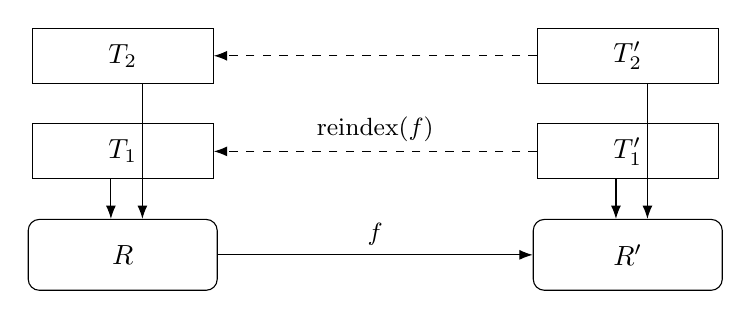
\begin{tikzpicture}[
      node distance=2.4cm,
      base/.style={rectangle,rounded corners,draw,minimum width=2.4cm,minimum height=0.9cm,align=center},
      tag/.style={rectangle,draw,minimum width=2.3cm,minimum height=0.7cm,align=center},
      >=Latex
    ]
    % Base objects
    \node[base] (R) {$R$};
    \node[base,right=4cm of R] (Rp) {$R'$};

    \draw[->] (R) -- node[above]{\small $f$} (Rp);

    % Fiber over R
    \node[tag,above=0.5cm of R] (T1) {$T_1$};
    \node[tag,above=0.5cm of T1] (T2) {$T_2$};

    % Fiber over R'
    \node[tag,above=0.5cm of Rp] (T1p) {$T'_1$};
    \node[tag,above=0.5cm of T1p] (T2p) {$T'_2$};

    % Projections over R
    \draw[->] ($(T1.south) + (-0.15cm,0)$) -- ($(R.north) + (-0.15cm,0)$);
    \draw[->] ($(T2.south) + (0.25cm,0)$)  -- ($(R.north) + (0.25cm,0)$);

    % Projections over R'
    \draw[->] ($(T1p.south) + (-0.15cm,0)$) -- ($(Rp.north) + (-0.15cm,0)$);
    \draw[->] ($(T2p.south) + (0.25cm,0)$)  -- ($(Rp.north) + (0.25cm,0)$);

    % Reindexing along f, fiber over R' -> fiber over R
    \draw[->,dashed] (T1p) -- node[above]{\small $\mathrm{reindex}(f)$} (T1);
    \draw[->,dashed] (T2p) -- (T2);

  \end{tikzpicture}
  \caption{Context tags as a fibration $\pi : \mathbf{CT} \to \mathbf{CEP}$.
    Each base record $R$ has a fiber of permitted tags above it.
    A morphism $f : R \to R'$ induces a reindexing between fibers,
    while the underlying canonical identity remains anchored in the base.}
  \label{fig:fibration-ctags}
\end{figure}
   % Diagrammatic intuition
% !TeX root = 00_cep_semantics.tex
\clearpage
\section*{Appendix E. Glossary for Non-Category Theory Readers}
\addcontentsline{toc}{section}{Appendix E. Glossary for Non-Category Theory Readers}

This appendix provides short, non-technical explanations of the categorical
concepts used in the paper.
The intention is to make the mathematical structure
of CEP more accessible to readers from computer science, data engineering,
public administration, and civic-technology communities.

% ------------------------------------------------------------
\subsection*{E.1 Categories}
A \emph{category} is a mathematical setting that describes:
\begin{itemize}
  \item some \textbf{objects} (things), and
  \item some \textbf{morphisms} (arrows) between them.
\end{itemize}

A category is like a directed graph with rules:
every arrow (morphism) has a source and target,
arrows can be composed,
and each object has an identity arrow that starts from the object, points back to the object, and does nothing.

The latin root \emph{morph} means "form" or "shape",
so a morphism is a way of changing the form of one object into another.

In CEP:
\begin{itemize}
  \item objects = record states,
  \item morphisms = valid record transformations (updates, amendments, joins).
\end{itemize}

Defining CEP as a category formalizes the idea of "things and the allowed changes between them".

% ------------------------------------------------------------
\subsection*{E.2 Functors}
A \emph{functor} is a mapping between categories that preserves structure.
It sends:
\begin{itemize}
  \item each object to another object, and
  \item each morphism to another morphism,
\end{itemize}
in a way that respects composition and identity.

In CEP, a functor often represents a pipeline stage, such as:
\begin{itemize}
  \item wrapping a payload in an envelope,
  \item normalizing noisy text into canonical components,
  \item assembling canonical strings.
\end{itemize}

Functors ensure that if a record evolves legally, its transformed
version evolves legally too.

\emph{Function} and \emph{functor} have the same root and similarities,
but different meanings:
functions map elements within sets,
while functors map objects and morphisms between categories.

% ------------------------------------------------------------
\subsection*{E.3 Natural Transformations}
A \emph{natural transformation} is a structured way of comparing two functors.
If functors are "processing stages", a natural transformation is a
systematic way to convert the output of one stage into the output of another.

In CEP, attestations are modeled as natural transformations:
\begin{itemize}
  \item the envelope functor produces a plain metadata wrapper,
  \item the attested-envelope functor produces a cryptographically validated wrapper.
\end{itemize}

Naturality expresses the idea:
\begin{quote}
  "Whether you process then attest, or attest then process,
  you end up with consistent provenance."
\end{quote}

% ------------------------------------------------------------
\subsection*{E.4 Monoidal Categories}
A \emph{monoidal category} is a category equipped with a notion of
"combining things".

Examples:
\begin{itemize}
  \item strings combine by concatenation,
  \item datasets combine by joining,
  \item workflows combine by sequencing.
\end{itemize}

Canonicalization is the process of converting data into a standard format,
most commonly by selecting a single, preferred output
to represent a piece of content that could have multiple versions.

Canonicalization in CEP is \emph{monoidal} because it combines
individual normalized components into a single canonical string
in a strictly deterministic order.

% ------------------------------------------------------------
\subsection*{E.5 Strict Monoidal Functors}
A \emph{strict monoidal functor} is a functor that preserves the
combination structure \emph{exactly}.

In CEP:
\begin{itemize}
  \item the order of pieces (name, address, date, jurisdiction)
        must always be preserved,
  \item no additional symbols or whitespace are introduced,
  \item the final output is the canonical string fed to the SHA-256 cryptographic hash function.
\end{itemize}

This strictness is what guarantees the stability of the SNFEI identifier.

% ------------------------------------------------------------
\subsection*{E.6 Oplax Functors}
An \emph{oplax functor} preserves structure in a weakened, direction-sensitive way.
The \emph{op} prefix indicates \emph{opposite} directionality and \emph{lax} indicates looseness.
An oplax functor therefore "loosens" structure in a specific direction and
allows "preservation up to a coherence map" rather than strict equality.
A coherence map is a controlled way of relating two structures that are not strictly equal.

It allows:
\begin{itemize}
  \item missing fields,
  \item lossy interpretations,
  \item mappings that preserve meaning but not full structure.
\end{itemize}

Jurisdictional adapters in CEP behave oplaxly because:
\begin{itemize}
  \item local data models may omit fields,
  \item global vocabularies may have stricter typing,
  \item some equivalences hold only "up to" a coherence rule.
\end{itemize}

Oplax behavior models "local autonomy with global convergence".
It means that local jurisdictions can adapt data flexibly
while still ensuring that the global system remains coherent and consistent.

% ------------------------------------------------------------
\subsection*{E.7 Pullbacks (Consistent Joins)}
A \emph{pullback} is the categorical notion of a \emph{consistent join}.

If two data sources both refer to the \emph{same entity or event},
the pullback constructs the most precise version of their agreement.

This formalizes CEP's guarantee that:
\begin{quote}
  Records may be joined only when they assert compatible facts.
\end{quote}

A pullback enables us to formally define the data fusion operation that
combines records from different schemas while preserving:
\begin{itemize}
  \item canonical identity,
  \item vocabulary-governed semantics,
  \item provenance constraints.
\end{itemize}

\emph{Data fusion} refers to the process of integrating multiple data sources
to produce more consistent, accurate, and useful information than that
provided by any individual source.

% ------------------------------------------------------------
\subsection*{E.8 Fibered Categories}
A \emph{fibered category} describes a setting where each object has a
family of additional structures "above it".

CEP is a fibered category.
In CEP:
\begin{itemize}
  \item the base category is $\mathbf{CEP}$,
  \item the fibers contain context tags (CTags).
\end{itemize}

This cleanly separates:
\begin{itemize}
  \item \textbf{identity} (in the base category), and
  \item \textbf{interpretation or annotation} (in the fiber).
\end{itemize}

CTags provide information about a record, without affecting the canonical SNFEI identifier.

% ------------------------------------------------------------
\subsection*{E.9 Universal Properties}
A \emph{universal property} describes an object that is "best" or "most canonical" for a specific purpose.

SNFEI behaves like a universal property construction because:

\begin{itemize}
  \item it is determined by a canonical string,
  \item it is invariant under allowed morphisms,
  \item any other identifier consistent with CEP's invariants must factor uniquely through this construction.
\end{itemize}

This is the mathematical justification enabling us to treat SNFEI
as a stable, verifiable, compositional global identifier.

  % ------------------------------------------------------------
  {\small
    \subsection*{E.10 Summary Table}
    \begin{center}
      \begin{tabular}{p{0.23\linewidth} p{0.35\linewidth} p{0.32\linewidth}}
        \toprule
        \textbf{Concept}        & \textbf{Intuition}       & \textbf{CEP Role}         \\
        \midrule
        Category                & Things, allowed changes  & Record states and updates \\
        Functor                 & Structure-preserving map & Normalization, envelopes  \\
        Natural transformation  & Coherent comparison      & Attestations              \\
        Monoidal category       & Combine things           & Canonical assembly        \\
        Strict monoidal functor & Combine exactly          & SNFEI stability           \\
        Oplax functor           & Weak structure map       & Jurisdiction adapters     \\
        Pullback                & Consistent join          & Merging record fragments  \\
        Fibered category        & Object annotations       & CTags above records       \\
        Universal property      & Optimal construction     & Identifier uniqueness     \\
        \bottomrule
      \end{tabular}
    \end{center}
  }

% ------------------------------------------------------------
\subsection*{E.11 Closing Note}
These notions are not introduced for abstraction's sake;
they express precisely and formally the structural guarantees
CEP requires to support interoperability, trust, and cross-jurisdiction governance.

These mathematical definitions allow the protocol to be:
\begin{itemize}
  \item modular in its design,
  \item formally verifiable in its behavior,
  \item capable of operating consistently even when sources use different schemas, vocabularies, or jurisdictional rules,
  \item and extensible to future domains.
\end{itemize}

By grounding CEP in category theory,
we provide a rigorous foundation for its design principles and operational claims.
   % Categorical Concepts for CEE
% !TeX root = 00P3_cee_verticals.tex

\clearpage
\section*{Appendix F. Supporting Categorical Terminology}
\addcontentsline{toc}{section}{Appendix F. Supporting Categorical Terminology}

This appendix defines categorical terms used in CEE that extend beyond the
foundational concepts in CEP Appendix~E. Readers unfamiliar with category
theory should consult CEP's glossary first for definitions of \emph{functor},
\emph{natural transformation}, \emph{monoidal category}, \emph{pullback},
and \emph{fibered category}.

\begin{description}[style=nextline,leftmargin=1.5cm]

  \item[Cartesianness]
        A property ensuring structured data can be ``pulled back'' along
        relationships without losing information. Cartesian structure guarantees
        that restricting a federal dataset to a state jurisdiction preserves all
        relevant relationships. See \emph{pullback} in CEP Appendix~E.

  \item[Compositionality]
        The principle that complex structures are built from simpler parts, with
        the meaning of the whole determined by the parts and how they combine.
        CEE's compositional design means evidence chains can be assembled from
        individual attestations.

  \item[Definedness]
        Whether an operation or relationship is valid for given inputs. Partial
        functions may be undefined for some inputs; CEE explicitly tracks
        definedness to distinguish ``no data'' from ``not applicable.''

  \item[Endofunction]
        A function from a set to itself. Update operations on entity state are
        endofunctions: they take a state and return a new state of the same type.

  \item[Fibered Category]
        A category equipped with a structure-preserving projection to a base
        category, allowing objects and morphisms to be indexed by elements of
        that base. In CEE, vertical domains are modeled as fibered categories over
        the CEP base category, enabling domain-specific semantics layered atop a
        shared canonical infrastructure. See \emph{fibered category} in CEP
        Appendix~E.

  \item[Fibered Structure]
        The organizational pattern induced by a fibered category, in which
        objects are grouped into fibers over a base category according to
        context or domain. In CEE, fibered structure allows vertical domains to
        specialize interpretation and evidence while remaining coherently
        anchored to the same underlying CEP entities and morphisms.

  \item[Functoriality]
        The property of preserving structure across transformations. A mapping
        is \emph{functorial} if it respects composition and identity---translating
        data between systems without corrupting accountability relationships.
        See \emph{functor} in CEP Appendix~E.

  \item[Lifting]
        Given a relationship at one level, finding a corresponding relationship
        at a higher level that projects down to it. Lifting allows inference of
        jurisdiction-level patterns from entity-level exchanges.

  \item[Monoidality]
        Structure allowing associative combination with a neutral element.
        Monetary values are monoidal under addition (zero is neutral). A mapping
        is \emph{monoidal} if it preserves this combining structure.
        See \emph{monoidal category} in CEP Appendix~E.

  \item[Naturality]
        A transformation is \emph{natural} if it works uniformly across all
        instances without depending on arbitrary choices. Natural mappings are
        canonical rather than ad hoc.
        See \emph{natural transformation} in CEP Appendix~E.

  \item[Oplaxity]
        A relaxed form of structure preservation where equations become directed
        inequalities. Oplax mappings allow ``preservation up to a coherence map''
        rather than strict equality, accommodating real-world data where
        composition may lose information.
        See \emph{oplax functor} in CEP Appendix~E.

  \item[Permutability]
        The property that certain operations can be performed in any order with
        the same result. Permutable operations simplify parallel processing and
        reduce coordination requirements in distributed systems.

  \item[Preordered]
        A set equipped with a reflexive and transitive relation (not necessarily
        antisymmetric). Time stamps and version numbers form preorders,
        generalizing ``earlier than'' or ``less detailed than.''

  \item[Quotienting]
        Collapsing distinctions by treating related elements as equivalent.
        Quotienting by jurisdiction aggregates city-level data into state-level
        summaries, treating individual cities as interchangeable for certain
        analyses.

\end{description}
   % Supporting categorical terminology

\bibliographystyle{plainnat}
\bibliography{bib_shared}
\end{document}
